\section{Categorization of Errors in Transformation Networks}

\todoLater{Discuss problem of default values, or more general \enquote{special cases}?}

\mnote{Categorization of errors}
In this section, we identify and categorize potential \emph{failures} that can occur when executing transformation networks, which are derived from the failure cases of the application algorithm discussed in \autoref{chap:orchestration}.
We consider the \emph{mistakes} and the resulting \emph{faults} in the transformation specifications, which a transformation developer can make.
The mistakes are specific for the introduced knowledge levels, thus we derive them from those levels.
We finally relate mistakes to the failures that can occur when transformation networks containing faults caused by those mistakes are still executed.

% In this section, we %first identify and 
% categorize potential \emph{failures} that can occur when executing \acp{BX} in a network to preserve consistency.
% We then consider \emph{mistakes} that a developer can make and that lead to \emph{faults} in the specifications of consistency and its preservation.
% \todo{Heißt der folgende Satz nicht, dass auf jeder Ebene genau ein Typ von Fehler auftreten kann?}
% We derive them from the specification levels introduced in \autoref{chap:properties:levels}, as each kind of mistake is specific for one of those levels.
% We finally relate the mistakes to the failures that can occur while executing the operationalization of a faulty consistency specification.
% That categorization forms our contribution \ref{contrib:issues}.
% In the following, we only discuss failures and their causing mistakes, but no strategies to solve or avoid them.
% Such strategies are discussed in \autoref{chap:prevention}.
%The identification and categorization in this section is based on argumentation. To show the correctness of identified mistakes, failures and their dependencies, we provide an appropriate evaluation in \autoref{sec:evaluation}.

%\todoHeiko{Introduce mistake, fault, failure} 

% \begin{itemize}
%     \item Define three essential abstraction levels in the development process
%     \item Levels depend on each other, so \emph{fulfillment} on one level is mandatory to investigate the next level
%     \item Mistakes on all levels may introduce failures in the execution of the operationalization of consistency constraint preservation
%     \item We summarize potential failures, identify their causes (mistakes and faults) and then categorize and relate them
% \end{itemize}

\subsection{Mistakes, Faults and Failures}

\mnote{Distinction of error types}
Errors in transformation networks can occur in different contexts, for example in terms of the transformation networks, more precisely the application algorithm, producing an incorrect result, or in terms of a transformation developer defining an erroneous transformation.
To be able to distinguish these contexts, we have already used the terms \emph{mistakes}, \emph{fault} and \emph{failure} with a short introduction of their distinction, as specializations of the general term \emph{error}.
They are supposed to describe erroneous or inappropriate knowledge of a developer (mistakes), erroneous implementations (faults) and erroneous execution results (failures).
These different types of errors depend on each other, as a mistake can lead to a fault, which can then lead to a failure.

\begin{properdescription}
    \item[Mistake:] \mnote{Erroneous knowledge}
    A mistake is made by a transformation developer. It is based on missing or erroneous knowledge about either the concrete transformation or the necessity to ensure certain properties. For example, the missing knowledge that transformations must be synchronizing leads to a mistake in the conceptualization of transformations as they do not ensure this required property. The missing knowledge that compatibility is required as well as the missing knowledge about the other transformations of a network can lead to the mistake that incompatible transformations are realized.
    If a transformation language abstracts from a conceptual level and relieves the developer from ensuring that no mistakes at that level are made, such mistakes can also be made by the transformation language developer and then manifest in a faulty implementation of the language. We do, however, not consider that case explicitly. 
    \item[Fault:] \mnote{Erroneous implementation}
    A fault is the manifestation of a mistake in the implementation of transformations. For example, the missing knowledge about the necessity to have synchronizing transformations can lead to the fault that the implementation does not properly match existing elements instead of creating new ones. A fault is, thus, always the consequence of a mistake. It is also made by a transformation developer, but can be seen within the implementation explicitly, whereas a mistake can only be detected by the fault in the implementation to which it led.
    \item[Failure:] \mnote{Manifestation of fault during execution}
    A failure occurs at execution time of transformations and is the manifestation of a fault when executing a faulty transformation network. A failure is the incorrect result of the execution of transformations. Whenever the transformations in a network have a faulty implementation, failures such as the termination in inconsistent states or non-termination of the application algorithm can occur. Since the occurrence of a failure depends on the scenario in which the transformations are executed, not every fault leads to a failure. On the other hand, a fault can also lead to several failures, e.g., because a transformation is executed multiple times.
\end{properdescription}

\mnote{Relation to other error notions}
Several similar terms like errors, mistakes, faults, bugs, defects and so on are used in software engineering and especially in software testing.
They are sometimes used interchangeably and sometimes with specific meanings.
One common notion is the distinction of faults, errors and failures in software testing, however also with different meanings, of which at least one is comparable to ours using the term \emph{error} for what we call \emph{mistake}.
We decided to avoid the overloaded term \emph{error} and make the human \emph{mistake} explicit.


\subsection{Possible Failure Types}
\label{chap:errors:categorization:failures}

\mnote{Essential failure types}
Failures are the manifestation of faults during transformation execution and thus the final result of mistakes made by a transformation developer.
A failure means that the execution of the transformation network or more precisely the application algorithm reached an unwanted state.
We have already discussed in \autoref{chap:orchestration:decidability:correctness_termination} that the application algorithm can fail by not implementing a correct application function, thus either returning models that are inconsistent or not terminating at all.
Additionally, the algorithm may fail to deliver consistent models by returning $\bot$.
Returning $\bot$ is actually desired behavior to deal with the undecidability of the orchestration problem.
It can, however, mask that the transformations in the network contain faults that lead to the algorithm not being able to find consistent models.

\mnote{Specialization options for failure types}
Termination in an inconsistent state, non-termination and returning $\bot$ already form the three general failure types that can occur when executing faulty transformations.
They can be further specialized in different dimensions, e.g., regarding determinism of inconsistent termination or regarding whether too many or too few elements (or combination of them) exist for being consistent, i.e., whether corresponding condition elements are missing or whether too many condition elements exist for which no consistent models can be found by adding further ones.
We did, however, find in previous work~\cite[Table~5.7]{saglam2020ma} that the distinction regarding elements does not provide any insights and benefits when tracing the failures back to the causal mistakes.
We do, however, consider \emph{duplications} as one specific additional failure type, which can finally lead to any of the other failures, depending on whether the application algorithm aborts or not.
Duplications of elements are of particular importance, because they are the essential manifestation of missing synchronization in transformations, as we have discussed in \autoref{chap:synchronization:achieving}.

\begin{figure}
    \centering
    \newcommand{\labelcolumnwidth}{4.5em}
\newcommand{\contentcolumnwidth}{7em}
\newcommand{\failurecolumnfactor}{1.65}
\newcommand{\rowdistance}{6em}

\begin{tikzpicture}[
    entry/.style={font=\small}
]

    
    \node[text depth=18em, minimum width=\contentcolumnwidth+\labelcolumnwidth, minimum height=20em] %, fill=lightgray!50]
    (errors) {\textbf{Mistakes}};
    \node[right=\contentcolumnwidth+0.5*\labelcolumnwidth of errors.center, anchor=center, text depth=18em, minimum width=\contentcolumnwidth, minimum height=20em] %, fill=lightgray!25] 
    (faults) {\textbf{Faults}};
    \node[right=(0.5+0.5*\failurecolumnfactor)*\contentcolumnwidth of faults.center, anchor=center, text depth=18em, minimum width=\failurecolumnfactor*\contentcolumnwidth, minimum height=20em] %, fill=lightgray!50] 
    (failures) {\textbf{Failures}};
    
    \node[below=5em of errors.north west, anchor=west, align=left, inner sep=0.7em] (transformation) {Level 1:\\ \emph{Transfor-}\\\emph{mation}};
    \node[below=\rowdistance of transformation.west, anchor=west, align=left, inner sep=0.7em] (relation) {Level 2:\\ \emph{Network}\\\emph{Relation}};
    \node[below=\rowdistance of relation.west, anchor=west, align=left, inner sep=0.7em] (rule) {Level 3:\\ \emph{Network}\\\emph{Rule}};
    
    \draw[thick] (errors.north west) -- ++(\labelcolumnwidth+2*\contentcolumnwidth+\failurecolumnfactor*\contentcolumnwidth, 0);
    \draw[very thin] ([yshift=0.5*\rowdistance, xshift=0.05*\contentcolumnwidth]transformation.west) -- ++(\labelcolumnwidth+0.9*\contentcolumnwidth,0);
    \draw[very thin] ([yshift=0.5*\rowdistance, xshift=\labelcolumnwidth+1.05*\contentcolumnwidth]transformation.west) -- ++(0.9*\contentcolumnwidth,0);
    \draw[very thin] ([yshift=0.5*\rowdistance, xshift=\labelcolumnwidth+2.05*\contentcolumnwidth]transformation.west) -- ++(\failurecolumnfactor*\contentcolumnwidth-0.1*\contentcolumnwidth,0);
    \draw[dashed, very thin] ([yshift=0.5*\rowdistance, xshift=0.05*\contentcolumnwidth]relation.west) -- ++(\labelcolumnwidth+0.9*\contentcolumnwidth,0);
    \draw[dashed, very thin] ([yshift=0.5*\rowdistance, xshift=0.05*\contentcolumnwidth]rule.west) -- ++(\labelcolumnwidth+0.9*\contentcolumnwidth,0);
    \draw[thick] (errors.south west) -- ++(\labelcolumnwidth+2*\contentcolumnwidth+\failurecolumnfactor*\contentcolumnwidth, 0);
    
    % ERRORS
    \node[entry, right=\labelcolumnwidth+0.5*\contentcolumnwidth of transformation.west, anchor=center, align=center] (error_transformation) {missing\\ synchronization};
    
    \node[entry, right=\labelcolumnwidth+0.5*\contentcolumnwidth of relation.west, anchor=center, align=center] (error_relation) {incompatible \\ constraint\\ knowledge};
    
    \node[entry, right=\labelcolumnwidth+0.5*\contentcolumnwidth of rule.west, anchor=center, align=center] (error_rule) {contradicting \\ options \\ selection};
    
    % FAULTS
    \node[entry, right=\contentcolumnwidth of error_transformation.center, anchor=center, align=center] (fault_matching) {missing \\ element\\ matching};
    \node[entry, below=5em of fault_matching.south, anchor=north, align=center] (fault_contradicting) {contradicting \\ element\\ generation / \\ change};
    
    % FAILURES
    \node[entry, right=(0.5+0.5*\failurecolumnfactor)*\contentcolumnwidth of fault_matching.north, anchor=north, align=center] (failure_duplications) {
        duplications\\
        \textbullet\ multiple instantiations\\
        \textbullet\ multiple insertions
    };
    
    \node[entry, below=1em of failure_duplications.south, anchor=north, align=center] (failure_termination) {
        inconsistent termination\\
        \textbullet\ deterministic\\
        \textbullet\ non-deterministic
    };
    
    \node[entry, below=1em of failure_termination.south, anchor=north, align=center] (failure_non_termination) {
        non-termination\\
        \textbullet\ alternation\\
        \textbullet\ divergence
    };
    
    \node[entry, below=1em of failure_non_termination.south, anchor=north, align=center] (failure_bot) {
        returning $\bot$
    };

    % ERROR -> FAULT
    \draw[-latex] ([xshift=-1.2em,yshift=0.6em]error_transformation.east) -- ([yshift=0.6em]fault_matching.west);
    
    \draw[-latex] ([xshift=-0.9em]error_relation.east) .. controls ++ (2.2em,0em) and ($(fault_contradicting.west)-(1.5em,-0.8em)$) .. ([yshift=0.8em]fault_contradicting.west);
    \draw[-latex] ([xshift=-0.5em]error_rule.east) .. controls ++ (2em,0em) and ($(fault_contradicting.west)-(1.5em,-0.3em)$) .. ([yshift=0.3em]fault_contradicting.west);
    
   
    % % FAULT -> FAILURE
    \draw[-latex] ([xshift=-0.3em]fault_matching.east) .. controls ++ (3em,0em) and ($(failure_duplications.west)-(1em,-1.1em)$) .. ([yshift=1.1em,xshift=2em]failure_duplications.west);
    
    \draw[-latex] ([xshift=-0.7em,yshift=0.8em]fault_contradicting.east) .. controls ++ (2.2em,0em) and ($(failure_termination.west)-(2.2em,-1.1em)$) .. ([yshift=1.1em,xshift=0em]failure_termination.west);
    \draw[-latex] ([xshift=-0.7em,yshift=0.5em]fault_contradicting.east) .. controls ++ (2em,0em) and ($(failure_non_termination.west)-(2em,-1.1em)$) .. ([yshift=1.1em,xshift=0em]failure_non_termination.west);
    \draw[-latex] ([xshift=-0.7em,yshift=0.2em]fault_contradicting.east) .. controls ++ (3em,0em) and ($(failure_bot.west)-(3em,0em)$) .. (failure_bot.west);

    \draw[-latex] ([xshift=-2em,yshift=1.1em]failure_duplications.east) -- ++(3em,0) |- (failure_bot.east);
    \draw[-latex] ($(failure_duplications.east)+(1em,-3.6em)$) -- ++(-0.9em,0);
    \draw[-latex] ($(failure_duplications.east)+(1em,-8.1em)$) -- ++(-2.2em,0);
    
\end{tikzpicture}
    %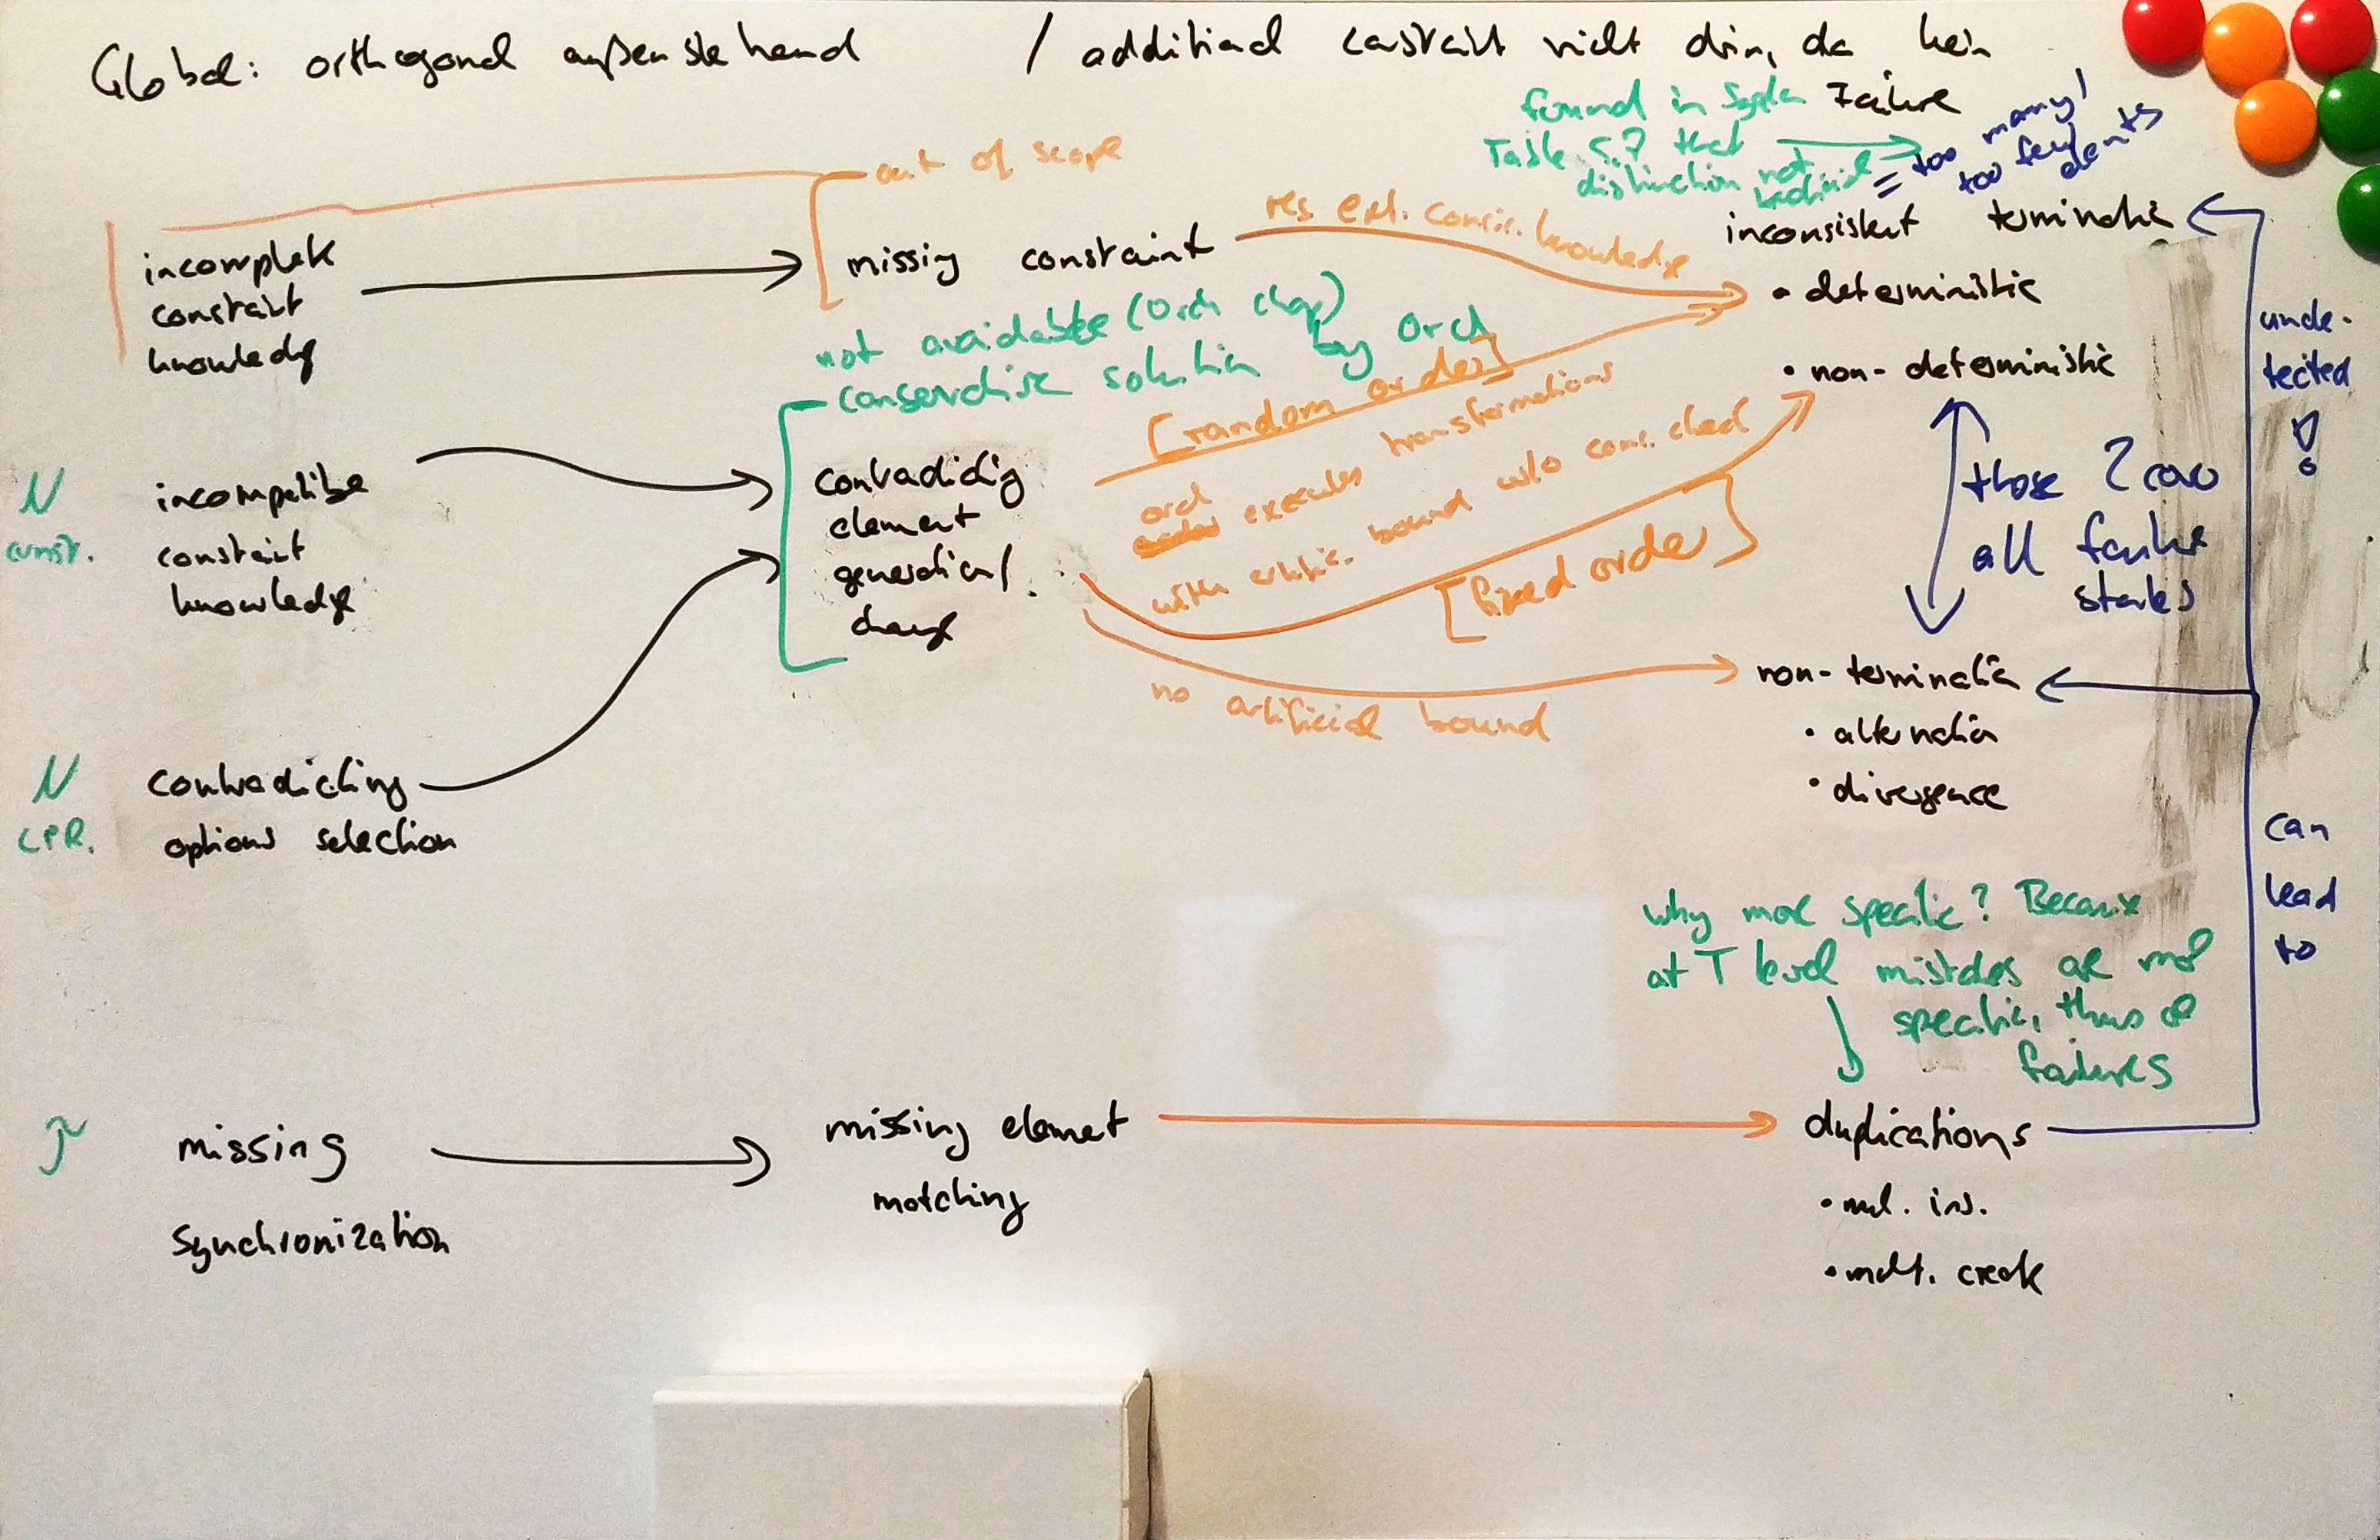
\includegraphics[width=\textwidth]{figures/correctness/errors/categorization.jpg}
    \caption[Categorization of mistakes, faults and failures]{Categorization of mistakes, faults and failures. Adapted from~\owncite{klare2019icmt}.}
    \label{fig:errors:categorization}
\end{figure}

\mnote{Failures depending on application algorithm}
In \autoref{fig:errors:categorization}, we depict the different failure types with their specializations, which we discuss in the following.
Note that we do not assume a specific application algorithm when discussing failures.
Whether a potential failure occurs or not highly depends on the used algorithm.
For example, using the provenance algorithm proposed in \autoref{chap:orchestration:algorithm} will neither lead to non-termination nor to inconsistent models, at least if the consistency check is implemented properly, but may only lead to returning $\bot$.
Having an artificial upper bound for the number of transformation executions, of course, always prevents from non-termination.
Only if transformations are executed without checking consistency afterwards or without defining an execution bound, the discussed failures can actually occur.
%In other cases, the actual failures are masked by the algorithm simply aborting and returning $\bot$.
Whenever an algorithm returns $\bot$, it can, however, be an indicator whether the algorithm fails because an artificial execution bound was reached or because a transformation cannot be applied anymore, because it is not able to process the given changes.
We will discuss that in \autoref{chap:errors:avoidance}.

% Mistakes in the specification of consistency, no matter on which of the specification levels, % (\autoref{sec:process:levels}),
% can lead to failures when executing the preservation of consistency according to that specification. % on an actual system. 
% Before identifying the causal mistakes, we first categorize the types of potential failures into three categories. We depict them in \autoref{fig:errors:categorization}.

We further distinguish the already discussed failure types as follows.
\begin{properdescription}
    \item[Inconsistent termination:] %\mnote{Termination in inconsistent states}
    Inconsistent termination means that the application algorithm terminates and the models it returns are inconsistent.
    This can only occur if the algorithm does not check the models yielded by the application of transformations in the order determined by the orchestration function for consistency.
    Furthermore it can terminate \emph{deterministically} or \emph{non-deterministically}, depending on whether each execution delivers the same inconsistent models or different ones, because different execution orders of the transformations are selected, which yield different inconsistent models.

    \item[Non-termination:] %\mnote{Non-termination in terms of alternation or divergence}
    Non-termination means that the application algorithm does not terminate, but executes transformations indefinitely without achieving a consistent state of the models.
    We can further distinguish between \emph{alternation} and \emph{divergence} as defined in \autoref{def:applyalternation}.
    Alternation means that the same model states are produced repeatedly, which can, for example, be because a feature, such as an attribute or reference, alternates between two or more values.
    In other cases, divergence occurs, which means that some feature values are changed indefinitely, such as a number counting up or a string being appended repeatedly, or an infinite number of elements is created.
    While an alternating algorithm can easily run endlessly, a diverging algorithm will abort at some point in time in many cases, because endless element creation or string concatenation can lead to an overflow of available memory.
    
    \item[Returning $\bot$:] %\mnote{Termination without yielding consistent models}
    The application algorithm may terminate and return $\bot$ to indicate that it was not able to find an orchestration that yields consistent models.
    This may either be because no such orchestration exists or can be found even though no mistakes were made, or because the transformation network actually contains faults that prevents the algorithm from finding a consistent orchestration.
    For example, if transformations are not synchronizing, the application algorithm will, in general, not be able to execute them in a way that they deliver consistent models.
    This kind of failure is different from the others, as it is intended behavior of the algorithm to return $\bot$ rather than returning inconsistent models or not terminating at all, but still it is not the intended result which may be caused by an actual mistake made by the transformation developer.

    \item[Duplications:] %\mnote{Element duplications as a special case leading to non-termiation or inconsistent termination}
    As a more specific failure case, we have introduced element duplications, which can especially arise if transformations are not synchronizing and thus do not match existing elements rather than creating new ones.
    We can further separate this into \emph{multiple instantiation}, which can occur because different consistency preservation rules instantiate an element multiple times, although all of them represent the same one, and \emph{multiple insertion}, which can occur because an element is inserted into a reference or attribute list several times, although it should be inserted only once. 
    In fact, such duplications can ultimately also lead to inconsistent termination, non-termination, or returning $\bot$, because either the algorithm returns after a finite number of transformation executions without checking consistency or checking it and returning $\bot$, or the transformations are not able to restore consistency for the models and the algorithm does thus not terminate.
    Duplications, however, represent a special case, which, as we will see in the evaluation in \autoref{chap:correctness_evaluation}, is one of the most important error cases for transformation networks.
    Thus, identifying such duplications in the generated models can ease finding the causal mistake in terms of missing synchronization.
\end{properdescription}

\mnote{Consistency checks problematic}
We have discussed that if an application algorithm checks consistency and has an artificial execution bound, it will only return $\bot$ rather than having any other failure, especially not the more specific duplications. Knowing the other failures and their relation to the causal mistakes is still important.
First, when a transformation network with such an application algorithm yields $\bot$ in most cases, there will likely be a fault in the transformation implementations.
Temporarily replacing the algorithm with a less restrictive one can help to find the reasons, because then, for example, duplications may be detectable that help to identify missing synchronization.
Second, in many transformation languages consistency relations are not represented explicitly, thus consistency checks are performed by executing the transformation and checking whether changes were performed.
Then, if transformations are non-synchronizing, they return an actually inconsistent state, which may, however, not be identified by the transformation as such.
This is due to the fact that those transformations do not expect the synchronization scenario and thus assume that consistency is achieved by construction, i.e., that changes must only be processed for one model and thus the models are consistent after executing the consistency preservation rules.

% If mistakes are made during the specification of consistency, no matter on which of the levels introduced in \autoref{sec:process:levels}, this can finally lead to failures in the consistency preservation executed on an actual system. Before identifying the causing mistakes, we first give an overview on the types of failures that may occur and separate them into three categories.\\[-0.7em]

% \compactsubsection{Termination in inconsistent states}
% \begin{enumerate}[topsep=4pt]
%     \item \emph{Deterministic:} The consistency preservation process can deterministically terminate in a state that is not consistent. % wrt. the defined consistency specification.
%     \item \emph{Non-deterministic:} Consistency preservation can non-deterministically terminate in an inconsistent state, depending on the execution order of the binary consistency preservation specifications. %in which the partial consistency preservation rules are executed.
% \end{enumerate}

% \compactsubsection{Non-termination}
% \begin{enumerate}[resume, topsep=4pt]
%     \item \emph{Alternating loops:} Consistency preservation can be non-terminating, alternating between two or more values in at least one feature (e.g. a number or a String alternating between two values).
%     \item \emph{Diverging loops:} Consistency preservation can be non-terminating, having at least one feature with a diverging value (e.g. a number counting up or down, a String being always appended).
% \end{enumerate}

% \compactsubsection{Duplications}
% \begin{enumerate}[resume, topsep=4pt]
%     \item \emph{Multiple instantiation:} An element can be instantiated multiple times by different consistency preservation specifications, although all of them represent the same element and thus should be the same. E.g. an element is created by transformations $\mathcal{M}_1 \rightarrow \mathcal{M}_2 \rightarrow \mathcal{M}_3$ and another is created by transformations $\mathcal{M}_1 \rightarrow \mathcal{M}_3$, although the same element is meant.
%     \item \emph{Multiple referencing:} An element may also be inserted into a non-containment reference or an attribute list several times, although the same element is meant, within the same situations as multiple instantiation can occur.
% \end{enumerate}


\subsection{Mistake and Fault Types}
\label{chap:errors:categorization:mistakes}

% Failures can occur because of different conceptual and technical mistakes.
% We do not consider technical mistakes, e.g., missing handling of null or comparable things.
% We do not consider conceptual mistakes regarding correctness of a single transformation (unidirectional). I.e., if a single transformation does not ensure consistency in one direction appropriately, we do not consider that a relevant mistake. Mistakes regarding synchronization, however (occurring with concurrent changes but not changes in one of the models), are relevant.
% We assume that transformations are correct, i.e., CPRs correct w.r.t. their relations

% Weitere Fehlertypen diskutieren / explizit ausschließen, insb. Implementierungsfehler, technische Fehler. Diese führen i.d.R. aber auch dazu, dass eine Transformation nicht korrekt ist.
% Wir nehmen wir Korrektheit einer Transformation an!
% In der Evaluation werden wir das noch entsprechend unterscheiden.

\mnote{Mistakes by specification levels}
Developers can make different kinds of mistakes at each of the specification levels, which lead to faults in the implementation and eventually to different kinds of failures during transformation execution.
In the following, we derive mistakes and faults from the specification levels, depicted in \autoref{fig:errors:categorization}.

\mnote{Excluded mistake types}
We explicitly focus on conceptual mistakes and faults concerned with the development of transformation networks.
This especially excludes two types of mistakes:
\begin{properdescription}
    \item[Technical mistakes:] We do not consider technical and careless mistakes that are due to misuse of the transformation language, a coding error such as a missing handling of null values, or comparable mistakes.
    \item[Transformation incorrectness:] We do not consider any kinds of mistakes that lead to incorrect transformations. We assume that transformations are correct, i.e., that the consistency preservation rules produce results that are consistent to their consistency relations. Thus any mistake related to the transformations handling changes in only one of the models are out of scope, as they are part of research regarding the individual bidirectional transformations on their own. Mistakes regarding synchronization of transformations, i.e., the case that changes were performed to both models, are, however, relevant.
\end{properdescription}
In fact, technical mistakes eventually lead to incorrectness of the transformations.


\subsubsection*{\LevelTransformation Level}

\mnote{Correctness by synchronizing transformations}
Correctness at the \leveltransformation level requires each transformation to be synchronizing.
We have discussed in \autoref{chap:synchronization:achieving} that the essential requirement to make ordinary transformations synchronizing is the matching of existing elements, because transformations that were not developed for the synchronization case do usually not assume elements to be already existing but to be either added by changes that are processed by the transformation or created by the transformation itself.

\mnote{Missing knowledge about synchronization}
The mistake a transformation developer can make at this level is not to consider that synchronization is necessary, potentially because he or she does not even know that it is necessary. Then the transformation may be correct but not synchronizing.
In the implementation, this manifests as the absence of necessary matchings of elements.
We have already discussed that this finally leads to the duplicate creation or insertion of model elements when executing such transformations.


\subsubsection*{\LevelNetworkRelation Level}

\mnote{Correctness by combination or individual}
The \levelnetworkrelation level concerns correctness of the consistency relations in a transformation network.
In general, we can distinguish two notions of correctness for them, as discussed in \autoref{chap:correctness:notions_correctness}.
First, relations must reflect an intended, probably informal notion of consistency.
If the relations miss to reflect constraints of that notion or if they reflect additional constraints that are not part of that notion, the relations may be considered incorrect.
Second, the relations must be compatible.
As discussed in \autoref{chap:compatibility}, this is necessary to enable the consistency preservation rules to find consistent models at all.
In the worst case, there may not be a single tuple of models that is consistent to all consistency relations when they are incompatible.

\mnote{Individual correctness irrelevant}
The first correctness notion, however, only concerns a single consistency relation rather than the combination of them.
We thus assume it to be correct, as we assume each transformation to already be correct.
Finally, such incorrectness would not even be interesting, because additional constraints do not lead to failures but, in the worst case, only lead to not finding consistent models although they exist, and missing constraints simply lead to inconsistent models, as the result does not fulfill the constraints of the existing, informal notion of consistency.

\mnote{Correctness requires compatibility}
The relevant correctness notion is the one of compatibility.
One or more transformation developers can make the mistake of having incompatible knowledge about the consistency constraints encoded into the transformations.
This, in consequence, leads to a fault in the implementation of transformations, which may perform a contradicting generation or modification of model elements, for which no orchestration of the transformations may yield consistent models.
Depending on the operation of the application algorithm, this can lead to different types of failures.
If the transformations are executed with an artificial execution bound, the algorithm will terminate with inconsistent models, which may be returned or not, depending on whether it checks consistency.
The inconsistency will be deterministic or not, according to whether the execution order of transformations is fixed or not.
If the algorithm does not implement such an artificial bound, such a fault can also lead to non-termination of the algorithm, because the execution of transformations will never lead to consistent models.
Finally, if the algorithm implements an artificial execution bound and consistency checks, it may also return $\bot$ in this case.

\subsubsection*{\LevelNetworkRule Level}

\mnote{No precise correctness notion}
The \levelnetworkrule level concerns correctness of the complete transformations of a network.
We did not give a precise definition of what this correctness means.
In \autoref{chap:orchestration}, we have discussed assumptions to transformations to enable an application function to solve the orchestration problem, which could be a reasonable correctness measure.
We have, however, also discussed that we cannot make any practical assumptions to the transformations such that they improve the ability of the application algorithm to find a consistent orchestration if it exists.

\mnote{Mistake possibility by contradicting options}
We only know from \autoref{chap:orchestration:decidability:restriction} that consistency relations providing multiple options for corresponding elements to consider models consistent can lead to consistency preservation rules that always select elements which are not in the overlap of those options between different transformations.
In consequence, if transformation developers decide to implement consistency preservation rules that make such contradicting selections or generations of elements, the transformations may fail due to the same reasons as discussed for the \levelnetworkrelation level.
In this case, the causing mistake is that the transformation developers make contradicting selections of available options to restore consistency.

\mnote{No complete mistakes overview}
We did not find and define a property that a transformation set and especially their consistency preservation rules have to fulfill and instead concluded to deal with the orchestration problem by means of a conservative application algorithm.
Thus, we cannot give a reasonable or even complete overview of potential mistakes transformation developers can make at this level.

% \subsubsection{Global Level}
% Regarding global consistency specifications for a set of model types, two basic mistakes can be made. 
% These mistakes concern compliance of the defined consistency specification with the actual notion of consistency between the involved model types.
% First, a specification can be incomplete (\emph{underspecified}), which means that some consistency constraints are missed. 
% As a result, the consistency specification according to \autoref{def:consistency_specification} would contain more tuples of models than are actually consistent to each other. 
% %%As a result, if one would define the consistency specification according to \autoref{def:consistency_specification}, more tuples of models would be in the relation than are actually consistent to each other. 
% %Incomplete consistency specifications can lead to \emph{false positives}, when investigating whether a given tuple of models is consistent or not.
% Another potential mistake are too restricted (\emph{overspecified}) consistency specifications, which means that additional, faulty consistency constraints are considered. 
% As a result, actually consistent tuples of models would be missing in the consistency specification according to \autoref{def:consistency_specification}. 
% %As a result, if one would define the consistency specification according to \autoref{def:consistency_specification}, actually consistent tuples of models would not be in the relation. 
% %This %, in contrast, 
% %can lead to \emph{false negatives}, because actually consistent models are identified as inconsistent.

% \begin{figure}[bt]
%     \centering
% %    \includegraphics[angle=-90, width=\textwidth]{figures/levels_overview.pdf}
%     \newcommand{\modeltypesize}{3.6em}
\newcommand{\modelsize}{0.3em}

\begin{tikzpicture}[
    model type/.style={draw, circle, minimum height=\modeltypesize},
    model/.style={draw, fill, circle, minimum height=\modelsize, inner sep=0},
    label distance=-0.2em,
    every label/.append style={font=\small},
    legend/.style={font=\footnotesize}
]

\foreach \level in {1,2,3} {
    \node[model type, label=265:{$\mathcal{M}_1$}] at (\level*3.45*\modeltypesize, 0) (L\level_MM1) {};
    \node[model, above left=0.25*\modeltypesize and 0.2*\modeltypesize of L\level_MM1.center, anchor=center] (L\level_MM1_M1) {};
    \node[model, right=0.3*\modeltypesize of L\level_MM1.center, anchor=center] (L\level_MM1_M2) {};
    \node[model, below left=0.25*\modeltypesize and 0.2*\modeltypesize of L\level_MM1.center, anchor=center] (L\level_MM1_M3) {};
    
    \node[model type, label=280:{$\mathcal{M}_2$}] at (\level*3.45*\modeltypesize+1.7*\modeltypesize, 0) (L\level_MM2) {};
    \node[model, above right=0.25*\modeltypesize and 0.2*\modeltypesize of L\level_MM2.center, anchor=center] (L\level_MM2_M1) {};
    \node[model, left=0.3*\modeltypesize of L\level_MM2.center, anchor=center] (L\level_MM2_M2) {};
    \node[model, below right=0.25*\modeltypesize and 0.2*\modeltypesize of L\level_MM2.center, anchor=center] (L\level_MM2_M3) {};
    
    \node[model type, label=190:{$\mathcal{M}_3$}] at (\level*3.45*\modeltypesize+0.85*\modeltypesize, -1.35*\modeltypesize) (L\level_MM3) {};
    \node[model, above=0.25*\modeltypesize of L\level_MM3.center, anchor=center] (L\level_MM3_M1) {};
    \node[model, below left=0.25*\modeltypesize and 0.1*\modeltypesize of L\level_MM3.center, anchor=center] (L\level_MM3_M2) {};
    \node[model, below right=0.05*\modeltypesize and 0.25*\modeltypesize of L\level_MM3.center, anchor=center] (L\level_MM3_M3) {};
}

% CONSISTENCY L1
\draw[consistency relation] (L1_MM1_M1) -- (L1_MM2_M1);
\draw[consistency relation] ($(L1_MM1_M1)!0.13!(L1_MM2_M1)$) -- (L1_MM3_M2);
\draw[consistency relation] (L1_MM1_M2) -- (L1_MM2_M2);
\draw[consistency relation] ($(L1_MM1_M2)!0.5!(L1_MM2_M2)$) -- (L1_MM3_M1);

% CONSISTENCY L2
\draw[consistency relation] (L2_MM1_M1) -- (L2_MM2_M1);
\draw[consistency relation] (L2_MM1_M1) -- (L2_MM3_M2);
\draw[consistency relation, dashed] (L2_MM2_M1) -- (L2_MM3_M2);
\draw[consistency relation] (L2_MM1_M2) -- (L2_MM2_M2);
\draw[consistency relation] (L2_MM1_M2) -- (L2_MM3_M1);
\draw[consistency relation] (L2_MM2_M2) -- (L2_MM3_M1);
%\draw[consistency relation, dash dot] (L2_MM2_M1) -- (L2_MM3_M3);

% CONSISTENCY L3
%\draw[consistency relation] (L3_MM1_M1) -- (L3_MM2_M1);
%\draw[consistency relation] (L3_MM1_M1) -- (L3_MM3_M2);
%\draw[consistency relation] (L3_MM2_M1) -- (L3_MM3_M2);
%\draw[consistency relation] (L3_MM1_M2) -- (L3_MM2_M2);
%\draw[consistency relation] (L3_MM1_M2) -- (L3_MM3_M1);
%\draw[consistency relation] (L3_MM2_M2) -- (L3_MM3_M1);

% USER CHANGE L3
\node[model, user changed element, above left=0.25*\modeltypesize and 0.2*\modeltypesize of L3_MM1.center, anchor=center] (L3_MM1_M1) {};
\node[model, user changed element, above right=0.25*\modeltypesize and 0.2*\modeltypesize of L3_MM2.center, anchor=center] (L3_MM2_M1) {};
\node[model, user changed element, below left=0.25*\modeltypesize and 0.1*\modeltypesize of L3_MM3.center, anchor=center] (L3_MM3_M2) {};
\draw[-latex, user changed element] (L3_MM1_M1) -- node[legend, above=0.2em] {$\Delta$} (L3_MM1_M2);

% CONSISTENCY PRESERVATION L3
\node[model, consistency changed element, right=0.3*\modeltypesize of L3_MM1.center, anchor=center] (L3_MM1_M2) {};
\node[model, consistency changed element, left=0.3*\modeltypesize of L3_MM2.center, anchor=center] (L3_MM2_M2) {};
%\node[model, consistency changed element, above=0.25*\modeltypesize of L3_MM3.center, anchor=center] (L3_MM3_M1) {};
\node[model, consistency changed element, below right=0.05*\modeltypesize and 0.25*\modeltypesize of L3_MM3.center, anchor=center] (L3MM3_M3) {};
\draw[-latex, consistency changed element] (L3_MM2_M1) -- node[legend, below right=-0.3em] {$\Delta$} (L3_MM2_M2);
%\draw[-latex, consistency changed element] (L3_MM3_M2) -- node[legend, below right=0 and -0.3em] {$\Delta$} (L3_MM3_M1);
\draw[-latex, consistency changed element] (L3_MM3_M2) -- node[legend, below] {$\Delta$} (L3_MM3_M3);
\draw[-latex, dashed, consistency changed element, thin] ($(L3_MM1_M1)!0.4!(L3_MM1_M2)$) to[bend left=15] node[legend, above] {$\mathit{CPS}_{\mathit{CS}_{1,2}}$} ($(L3_MM2_M1)!0.4!(L3_MM2_M2)$);
%\draw[-latex, dashed, consistency changed element, very thin] ($(L3_MM1_M1)!0.4!(L3_MM1_M2)$) to[bend right=15] ($(L3_MM3_M2)!0.4!(L3_MM3_M1)$);
\draw[-latex, dashed, consistency changed element, very thin] ($(L3_MM1_M1)!0.4!(L3_MM1_M2)$) to[bend right=15] node[legend, below left=0.5em and -0.5em] {$\mathit{CPS}_{\mathit{CS}_{1,3}}$} ($(L3_MM3_M2)!0.4!(L3_MM3_M3)$);

% CS LABELS
\node[consistency related element, above left=1.5em and -0.1em of L1_MM3.north, anchor=east, font=\footnotesize] {$\mathit{CS}$};
\node[consistency related element, above left=0.1em and 1.6em of L2_MM3, anchor=center, font=\footnotesize] {$\mathit{CS}_{1,3}$};
\node[consistency related element, above right=0.4em and 1.2em of L2_MM3, anchor=center, font=\footnotesize] {$\mathit{CS}_{2,3}$};
\node[consistency related element, above right=0.8em and 0.25*\modeltypesize of L2_MM1.east, anchor=south, font=\footnotesize] {$\mathit{CS}_{1,2}$};
%\node[consistency related element, above left=0.4em and 1.8em of L3_MM3, anchor=center, font=\footnotefont] {$CS_{1,3}$};
%\node[consistency related element, above right=0.4em and 1.4em of L3_MM3, anchor=center, font=\footnotefont] {$CS_{2,3}$};
%\node[consistency related element, above right=0.8em and 0.25*\modeltypesize of L2_MM1.east, anchor=south, font=\footnotefont] {$CS_{1,2}$};

% LEVEL LABELS
\node[anchor=north] (level1_label) at ([yshift=1.15*\modeltypesize]$(L1_MM1)!0.5!(L1_MM2)$) {Level 1: \emph{Global}};
\node[anchor=north] (level2_label) at ([yshift=1.15*\modeltypesize]$(L2_MM1)!0.5!(L2_MM2)$) {Level 2: \emph{Modularization}};
\node[anchor=north] (level3_label) at ([yshift=1.15*\modeltypesize]$(L3_MM1)!0.5!(L3_MM2)$) {Level 3: \emph{Operationalization}};

\coordinate (legend_anchor) at ([yshift=-0.2*\modeltypesize]L2_MM3.south);

\node[matrix, left=-0.2em of legend_anchor, anchor=north east, outer sep=0em, column sep=0.15em, row sep=-0.4em] (legend_left) {
    \node[model, anchor=center] (model_legend) {}; &
    \node[legend, anchor=west] {model of model type $\mathcal{M}_x$}; \\
    %
    \node[model, user changed element, anchor=center] (user_changed_model_legend)  {}; &
    \node[legend, anchor=west] {consistent models before user change}; \\
    %
    \node[model, consistency changed element, anchor=center] (consistency_preserved_model_legend)  {}; &
    \node[legend, anchor=west] {consistent models after consistency preservation}; \\
};

\node[matrix, left=0.2em of legend_anchor, anchor=north west, column sep=0.15em, row sep=-0.4em] (legend_right) {
    \draw[consistency relation] (0,0.25em) -- (1em,0.25em);
    \draw[consistency relation] (0.5em,0.25em) -- (0.5em,-0.2em); &
    \node[legend, consistency related element, anchor=west] {element of consistency specification}; \\% $\mathit{CS}$}; \\
    % 
    \draw[-latex, user changed element] (0,0) -- (1em,0); &
    \node[legend, user changed element, anchor=west] {user change introducing inconsistency}; \\
    %
    \draw[-latex, consistency changed element] (0,0) -- (1em,0); &
    \node[legend, consistency changed element, anchor=west, align=left] {execution of consistency preservation specification};\\ % $\mathit{CPS}_{\mathit{CS}}$}; \\
};
\coordinate (legend_left_dummy) at ([xshift=-0.3em]legend_left.west);
\node[draw=darkgray, inner sep=0em, fit=(legend_left_dummy)(legend_left)(legend_right)] {};

\end{tikzpicture}

%     \caption{Examples for Mistakes on Different Specification Levels}
%     \label{fig:errors:mistakes_specification_levels}
% \end{figure}

% \subsubsection{Modularization Level}
% When developers modularize the global consistency specification by defining binary consistency specifications, these modular specifications can be non-compliant with the global one. 
% Two kinds of mistakes, similar to those at the global level, can be distinguished, regarding compliance of modular and global specifications. %, but regarding compliance of modular and global specifications rather than between the global specification and the actual notion of consistency.
% First, modular consistency specifications can be incomplete (\emph{underspecified}), so that there are global constraints which are not covered by them. 
% The modular consistency specifications $\mathit{CS}_{1,2}$, $\mathit{CS}_{2,3}$ and $\mathit{CS}_{1,3}$ in \autoref{fig:errors:mistakes_specification_levels} are incomplete if, and only if,
% %For three model types $\mathcal{M}_1, \mathcal{M}_2$ and $\mathcal{M}_3$ with a global consistency specification $\mathit{CS}$, the binary specifications $\mathit{CS}_{1,2}$, $\mathit{CS}_{2,3}$ and $\mathit{CS}_{1,3}$, as depicted in \autoref{fig:levels_overview} are underspecified if, and only if,
% %\todoHeiko{Hier die Grafik aus dem Level-Kapitel übernehmen}
% \begin{align*}
%     & \exists M_1, M_2, M_3 : \\
%     & \hspace{1em} (M_1, M_2) \in \mathit{CS}_{1,2} \land (M_2, M_3) \in \mathit{CS}_{2,3} \land (M_1, M_3) \in \mathit{CS}_{1,3} \land (M_1, M_2, M_3) \not\in \mathit{CS}
% \end{align*}
% This finally leads to \emph{false positives} when investigating whether a given tuple of models is consistent regarding the global specification. %as actually inconsistent models (regarding the global specification) are identified as consistent. %investigating whether a given set of models is consistent regarding the global specification or not, because actually inconsistent models regarding $\mathit{CS}$ are consistent according to all modular relations $\mathit{CS}_{1,2}$, $\mathit{CS}_{2,3}$ and $\mathit{CS}_{1,3}$.
% %This finally leads to \emph{false positives} when investigating whether a given set of models is consistent regarding the global specification or not, because actually inconsistent models regarding $CS$ are consistent according to all modular relations $\mathit{CS}_{1,2}$, $\mathit{CS}_{2,3}$ and $\mathit{CS}_{1,3}$.
% %\todoHeiko{Das folgende eher zu Avoidance Strategy? Überlapp vorhanden?}
% %Such incomplete specifications can especially occur if constraints between two types of models are not expressed at all (so the consistency specification covers all model pairs), but are only transitively defined over two or more other relations. 
% %For example, if $\mathit{CS}_{1,3}$ shall be omitted and transitively expressed across $\mathit{CS}_{1,2}$ and $\mathit{CS}_{2_3}$, the following must hold:
% % \begin{align*}
% %     & \forall M_1 \in \mathcal{M}_1 : \forall M_2 \in \mathcal{M}_2 : \forall M_3 \in \mathcal{M}_3 : \\
% %     & \hspace{1em} \mathit{CS}(M_1, M_2, M_3) \iff \mathit{CS}_{1,2}(M_1, M_2) \land \mathit{CS}_{2,3}(M_2, M_3)
% % \end{align*}
% %\begin{align*}
%     %& \forall M_1, M_2, M_3 : (M_1, M_2, M_3) \in \mathit{CS} \Leftrightarrow (M_1, M_2) \in \mathit{CS}_{1,2} \land (M_2, M_3) \in \mathit{CS}_{2,3}
% %\end{align*}
% %If this transitive relation misses or is even unable to express certain direct constraints, inconsistent models would be identified as consistent. %\todoHeiko{Das transitive muss man wohl an einem Beispiel erklären, am besten Ref. zu Intro}
% Modular consistency specifications cannot only be incomplete because of an actual specification mistake, but also because of $n$-ary relations on the global level that cannot be expressed by a set of binary relations.
% We excluded that case by our assumption made in \autoref{chap:properties:levels}, as otherwise a modularization into binary relations would not be possible at all.
% If such cases have to be supported, the modularization would have to be extended to also consider $n$-ary relations.

% Second, a modular specification can be too restricted (\emph{overspecified}) regarding the global consistency specification if additional constraints are added. 
% The modular consistency specifications in \autoref{fig:errors:mistakes_specification_levels} are overspecified if,and only if
% \begin{align*}
%     & \exists M_1, M_2, M_3 : \\
%     & \hspace{1em} (M_1, M_2, M_3) \in \mathit{CS} \land \big[ (M_1, M_2) \not\in \mathit{CS}_{1,2} \lor (M_2, M_3) \not\in \mathit{CS}_{2,3} \lor (M_1, M_3) \not\in \mathit{CS}_{1,3} \big]
% \end{align*}
% In \autoref{fig:errors:mistakes_specification_levels}, omitting the dashed relation in $\mathit{CS}_{2,3}$ would lead to such an overspecifiation.
% Overspecifications lead to additional constraints regarding the global specification, but also, and more severe, to contradicting constraints regarding other modular specifications.
% In case of contradictions, the modular consistency specifications cannot be fulfilled at the same time.
% In such a case, the graph of consistency relations %, as shown in \autoref{fig:mistakes_specification_levels}, 
% would contain no cycles, i.e. sets of models that are consistent to each other.
% We have discussed an example for such contradicting specifications %in the motivating example 
% in \autoref{chap:properties:levels}, where constraints for transferring an employee name contradicted. % contains contradicting constraints for transferring the name. % to other types of models.
% %In this case, when several binary specifications are combined to keep multiple models consistency, the resulting fault are incompatible binary specifications in the sense that different relations cannot hold at the same time because they are based on different global consistency specifications.
% Such mistakes lead to \emph{false negatives} as actually consistent models (regarding the global specification) are identified as inconsistent. %, when investigating whether a given set of models is consistent regarding the global specification or not, because actually consistent models regarding $\mathit{CS}$ are not consistent according to the modular relations $\mathit{CS}_{1,2}$, $\mathit{CS}_{2,3}$ and $\mathit{CS}_{1,3}$.

% %\begin{itemize}
%     %\item inadequate structure
%     %\item missing knowledge about other modular relation
% %\end{itemize}

% \subsubsection{Operationalization Level}
% The types of mistakes that can be made at the operationalization level are different from those at the other levels, because this level does not concern the definition of consistency specifications (\autoref{def:consistency_specification}), but of consistency \emph{preservation} specifications (\autoref{def:consistency_preservation_specification}).
% Such specifications are faulty if no composition of them exists that returns a consistent tuple of models for each possible change. % it does not lead to a consistent state after making modifications to a consistent tuple of models.
% In \autoref{fig:errors:mistakes_specification_levels}, an exemplary application of a single consistency preservation specification is depicted that leads to models that are not consistent according to the (global and modular) consistency specifications.
% %If no concatenation of CPSs exists that finally returns a consistent set of models for each possible change, the specifications are faulty.
% Let $\mathcal{CPS}$ be a set of consistency preservation specifications  %, e.g. $\mathcal{CPS} := \{\mathit{CPS}_{1}, \ldots, \mathit{CPS}_{m}\}$
% for the binary consistency specifications $\mathcal{CS}$ % := \{\mathit{CS}_{1,2}, \mathit{CS}_{2,3}, \mathit{CS}_{1,3}\}$ %(where there can be more than one consistency preservation specifications for each consistency specification) 
% %in \autoref{fig:mistakes_specification_levels}. %, metamodels $\mathcal{M}_0, \ldots, \mathcal{M}_n$, 
% and
% let $\mathfrak{M}_{\mathcal{CS}}$ be the set of model tuples that are consistent regarding $\mathcal{CS}$ (cf. \autoref{chap:properties:terminology}). 
% The consistency preservation specifications are faulty if, any only if,
% % \begin{align*}
% %     & \exists M_0, M'_0 \in \mathcal{M}_0, M_1, M'_1 \in \mathcal{M}_1, M_2, M'_2 \in \mathcal{M}_2 : \forall \mathit{CPS}_0, \ldots, \mathit{CPS}_k \in \mathcal{CPS} : \\
% %     & \hspace{1em} ((M_0, M''_0), (M_1, M''_1), (M_2, M''_2)) = \mathit{CPS}_0 \circ \dots \circ \mathit{CPS}_k((M_0, M'_0), (M_1, M'_1), (M_2, M'_2)) \\
% %     & \hspace{1em} \Rightarrow \exists \mathit{CS}_{i,j} \in \mathcal{CS} : \neg \mathit{CS}_{i,j}(M''_i, M''_j)
% % %    & \exists M_0, M'_0 \in \mathcal{M}_0, \ldots M_n, M'_n \in \mathcal{M}_n : \nexists \mathit{CPS}_0, \ldots, \mathit{CPS}_k \in \mathcal{CPS} : \\
% % %    & \hspace{1em} ((M_0, M''_0), \dots, (M_n, M''n)) := \mathit{CPS}_0 \circ \dots \circ \mathit{CPS}_k((M_0, M'_0), \dots, (M_n, M'_n)) \\
% % %    & \hspace{1em} \land \exists \mathit{CS}_{i,j} \in \mathcal{CS} : \neg \mathit{CS}_{i,j}(M''_i, M''_j)
% % \end{align*}
% \begin{align*}
%     & \exists (M_1, \dots, M_n) \in \mathfrak{M}_{\mathcal{CS}}, (M'_1, \dots, M'_n) \in \mathcal{M}_1 \times \dots \times \mathcal{M}_n: \forall \mathit{CPS}_1, \ldots, \mathit{CPS}_k \in \mathcal{CPS} : \\
%     %& \exists M_1, M'_1 \in \mathcal{M}_1, \dots, M_n, M'_n \in \mathcal{M}_n : \forall \mathit{CPS}_1, \ldots, \mathit{CPS}_k \in \mathcal{CPS} : \\
%     & \hspace{1em} \mathit{CPS}_1 \circ \dots \circ \mathit{CPS}_k \big((M_1, M'_1), \dots, (M_n, M'_n) \big) = \big( (M_1, M''_1), \dots, (M_n, M''_n) \big)\\
%     & \hspace{2em} \land \exists \mathit{CS}_{i,j} \in \mathcal{CS} : (M''_i, M''_j) \notin \mathit{CS}_{i,j}
% %    & \exists M_0, M'_0 \in \mathcal{M}_0, \ldots M_n, M'_n \in \mathcal{M}_n : \nexists \mathit{CPS}_0, \ldots, \mathit{CPS}_k \in \mathcal{CPS} : \\
% %    & \hspace{1em} ((M_0, M''_0), \dots, (M_n, M''n)) := \mathit{CPS}_0 \circ \dots \circ \mathit{CPS}_k((M_0, M'_0), \dots, (M_n, M'_n)) \\
% %    & \hspace{1em} \land \exists \mathit{CS}_{i,j} \in \mathcal{CS} : \neg \mathit{CS}_{i,j}(M''_i, M''_j)
% \end{align*}
% %\todoHeiko{Das ist nicht so schön, weil nicht klar ist, welche CS to welcher CPS gehört und so}
% %This means that there can be changes for which no execution of consistency preservation specifications is able to properly restore consistency. 

% In practice, mistakes at the operationalization level occur due to missing identification of equal elements in different consistency preservation specifications. 
% In our motivational example (\autoref{fig:properties:motivational_example}), %consider that an employee is created in the scheduling system for an employee created in the task management system after introducing one in the personnel management system.
% consider that an employee is created in the personnel management system, transformed to the task management system and from that to the scheduling system.
% The additional direct specification between personnel management and scheduling system has to consider the already created employee rather than instantiating a new one.
% %We consider %this case and 
% %options to avoid such problems in \autoref{sec:avoiding:matching}.
% %In our example, if a class is created in Java after creating a UML class for a ADL component through appropriate consistency preservation specifications and the consistency preservation specification between ADL and Java also defines the creation of a class in Java, it is necessary that the already existing class is considered rather than creating a new class. We will consider this case and options to avoid such problems in \autoref{sec:avoiding:matching}.

% % \begin{itemize}
% %     \item unknown connection of elements in consistency specifications
% %     \item Really, really make an example here, to distinguish from modularization level!!
% % \end{itemize}

% %In the following, we call all mistakes on modularization and operationalization level \emph{interoperability issues}, as they are all concerned with modularized specifications that have to interoperate. 


\subsection{Causal Chains}

\mnote{Mistakes, faults, failures dependencies}
We have already discussed the relevant causal chains between mistakes, faults and failures when introducing the relevant mistake types.
The full overview of these dependencies is given in \autoref{fig:errors:categorization}.
Mistakes at the \levelnetworkrelation and \levelnetworkrule levels can always lead to any kind of failure, namely non-termination, inconsistent termination, or returning $\bot$, depending on how the application algorithm operates.
Thus, these dependencies do not give an insights regarding which mistakes may have caused an occurring failure.
Mistakes at the \leveltransformation level, however, produce a specific kind of failure that can be distinguished from the general failure types.
Thus, knowing these causal chains is especially useful for identifying mistakes at the \leveltransformation level.
We further discuss the detection and avoidance of mistakes in the subsequent section.

\begin{figure}
    \centering
    \newcommand{\hdistance}{7em}
\newcommand{\classwidth}{6em}

\newcommand{\classdistance}{5em}
\newcommand{\objectwidth}{6.3em}

\begin{tikzpicture}[
    consistency preservation/.style={-latex, consistency changed element, font=\small},
    user change/.style={-latex, user changed element, font=\small},
    legend/.style={font=\footnotesize},
    mininode/.style={inner sep=.25em},
]

% Person
\umlclassvarwidth{person}{}{Person\sameheight}{
firstname\\
lastname
}{\classwidth}

% Employee
\umlclassvarwidth[,above right=1.5em and \hdistance of person.north east, anchor=south]{employee}{}{Employee\sameheight}{
name
}{\classwidth}

\umlclassvarwidth[,below right=1.5em and \hdistance of employee.south, anchor=north west]{resident}{}{Resident\sameheight}{
name
}{\classwidth}


% CONSISTENCY RELATIONS
\draw[consistency relation] (person.north) |- node[pos=0, above left] {$p$} node[pos=0.75, above] {$\consistencyrelation{CR}{PE}$} node[pos=1, above left] {$e$} (employee.west);
\draw[consistency relation] (employee.east) -| node[pos=0, above right] {$e$} node[pos=0.3, above] {$\consistencyrelation{CR}{ER}$ / $\consistencyrelation{CR}{ER}'$} 
node[pos=1, above right] {$r$} (resident.north);
\draw[consistency relation] (resident.west) -- node[pos=0, below left] {$r$} node[pos=0.5, below] {$\consistencyrelation{CR}{PR}$ / $\consistencyrelation{CR}{PR}'$} node[pos=1, below right] {$p$} (resident.west-|person.east);

%\draw[consistency relation 2] (person.east) -- node[pos=0, below right] {$p$} ++(0.35*\hdistance,0) -- node[pos=0, right=0.5em] {$R_{PER}$} node[pos=1, above left] {$e$} ([yshift=1em]employee.south west);
%\draw[consistency relation 2, ->] ([xshift=0.35*\hdistance]person.east) -- node[pos=1, below left] {$r$} ([yshift=-1em]resident.north west);

% \node[consistency related element 2, below left=5em and 2.5em of person.south west, anchor=north west] (relations1) {
% $\begin{aligned}
%     R_{PER} =\; &
%             \setted{\tupled{p,e,r} \mid \\
%             & p.firstname + "\text{\textvisiblespace}" + p.lastname = e.name = r.name\\
%             & \land p.address = r.address%\\
%             %& 
%             \land p.income = e.salary\\
%             & \land e.socsecnumber = r.socsecnumber
%         }
% \end{aligned}$
% };

%\node[consistency related element, below=0.5em of relations1.south west, anchor=north west] {
\node[consistency related element, below left=1.2em and 0em of person.south west, anchor=north west, inner sep=0em] {
$\begin{aligned}
    \consistencyrelation{CR}{PE} =\; &
            \setted{\tupled{p,e} \mid %\\
            %& 
            \mathvariable{p.firstname} + "\text{\textvisiblespace}" + \mathvariable{p.lastname} = \mathvariable{e.name}%\\
            %& \land p.income = e.salary
        }\\[0.3em]
    \consistencyrelation{CR}{PR} =\; &
            \setted{\tupled{p,r} \mid %\\
            %& 
            \mathvariable{p.firstname} + "\text{\textvisiblespace}" + \mathvariable{p.lastname} = \mathvariable{r.name}%\\
            %& \land p.address = r.address
        }\\
    \consistencyrelation{CR}{PR}' =\; &
            \setted{\tupled{p,r} \mid %\\
            %& 
            \mathvariable{p.lastname} + "\text{\textvisiblespace}" + \mathvariable{p.firstname} = \mathvariable{r.name}%\\
            %& \land p.address = r.address
    }\\[0.3em]
    \consistencyrelation{CR}{ER} =\; &
            \setted{\tupled{e,r} \mid %\\
            %& 
            \mathvariable{e.name} = \mathvariable{r.name}%\\
            %& \land e.socsecnumber = r.socsecnumber
        }\\
    \consistencyrelation{CR}{ER}' =\; &
            \setted{\tupled{e,r} \mid %\\
            %& 
            \mathvariable{e.name.toLower} = \mathvariable{r.name}%\\
            %& \land e.socsecnumber = r.socsecnumber
        }
\end{aligned}$
};

% % LEGEND
% \coordinate (legend_anchor) at ([xshift=1.5*\classwidth,yshift=-2.7*\classdistance]employee);

% \node[draw=darkgray, matrix, legend, nodes=mininode, below=0em of legend_anchor, anchor=north, outer sep=0, inner sep=0.4em, column sep=0.2em, row sep=-0.2em] (legend) {
%     \draw[consistency relation] (0,0) -- (1.4em,0); &
%     \node[consistency related element, anchor=west] {consistency constraint}; \\
%     %
%     \draw[-latex, user changed element] (0,0) -- (1.4em,0); &
%     \node[user changed element, anchor=west] {user change}; \\
%     %
%     \draw[-latex, consistency changed element] (0,0) -- (1.4em, 0); &
%     \node[consistency changed element, anchor=west, align=left] (legend_cpr_label) {consistency preservation};\\
% };

\end{tikzpicture}


%    \includegraphics[angle=270, width=\textwidth]{figures/mistakes_examples_employee.pdf}
    \caption[Adaptation of consistency relations from running example]{Adaptation of consistency relations from the extended running example in \autoref{fig:compatibility:three_persons_example_extended}. Adapted from~\owncite[Figure 5]{klare2019icmt}.}
    \label{fig:errors:mistake_effects_example_metamodels}
\end{figure}

\begin{figure}
    \centering
    \newcommand{\hdistance}{7em}
\newcommand{\classwidth}{6em}

\newcommand{\classdistance}{5em}
\newcommand{\objectwidth}{6.3em}

\begin{tikzpicture}[
    consistency preservation/.style={-latex, consistency changed element, font=\small},
    user change/.style={-latex, user changed element, font=\small},
    legend/.style={font=\footnotesize},
    mininode/.style={inner sep=.25em},
]

% LEVEL 1 ERROR
\coordinate (failure_l1_anchor) at (0,0);
\node[above=0.5em of failure_l1_anchor] {\textbf{\LevelTransformation Level Mistake} ($R_{PE}, R_{PR}, R_{ER}$)};

\umlobjectvarwidth[, fill=white, below=0 of failure_l1_anchor, anchor=north]{l1_employee}{}{
: Employee}{
name="Alice Avid"
}{\objectwidth}

\umlobjectvarwidth[, fill=white, below left=0.4*\classdistance and \classdistance+\classwidth of l1_employee.north, anchor=north] {l1_person}{}{
: Person}{
firstname="Alice"
lastname="Avid"
}{\objectwidth}

\umlobjectvarwidth[, fill=white, above right=1em and 2*\classdistance+2*\classwidth of l1_person.center, anchor=south] {l1_resident}{}{
: Resident}{
name="Alice Avid"
}{\objectwidth}

\umlobjectvarwidth[, fill=white, above right=0.5em and 2*\classdistance+2*\classwidth of l1_person.center, anchor=north] {l1_resident_duplicate}{}{
: Resident}{
name="Alice Avid"
}{\objectwidth}

\umlhuman{l1_human}{at ([xshift=1em, yshift=3em]l1_person.north west)}{user changed element}{}{0.5}
\draw[user change] ([xshift=1em,yshift=1.8em]l1_person.north west) -- node[right, align=center] {1. +} ([xshift=1em]l1_person.north west);
\draw[consistency preservation] ([yshift=1em]l1_person.east) -- node[above] {2. +} ([yshift=0em]l1_employee.west);
\draw[consistency preservation] (l1_employee.east) -- node[above] {3. +} (l1_resident.west);
\draw[consistency preservation] (l1_resident_duplicate.west-|l1_person.east) -- node[below] {4. +} (l1_resident_duplicate.west);


% LEVEL 2 ERROR
\coordinate (failure_l2_anchor) at ([yshift=-1.8*\classdistance]failure_l1_anchor);
\node[above=0.5em of failure_l2_anchor] {\textbf{\LevelNetworkRelation Level Mistake} ($R_{PE}, R_{PR}, R_{ER}'$)};

\umlobjectvarwidth[, fill=white, below=0 of failure_l2_anchor, anchor=north]{l2_employee}{}{
: Employee}{
name="Alice Avid"
}{\objectwidth}

\umlobjectvarwidth[, fill=white, below=0.7*\classdistance of l2_employee.north, anchor=north]{l2_employee2}{}{
: Employee}{
name="alice avid"
}{\objectwidth}

\umlobjectvarwidth[, fill=white, below left=0.4*\classdistance and \classdistance+\classwidth of l2_employee.north, anchor=north] {l2_person}{}{
: Person}{
firstname="Alice"
lastname="Avid"
}{\objectwidth}

\umlobjectvarwidth[, fill=white, below=0.9*\classdistance of l2_person.north, anchor=north]{l2_person2}{}{
: Person}{
firstname="alice"
lastname="avid"
}{\objectwidth}

\umlobjectvarwidth[, fill=white, right=2*\classdistance+2*\classwidth of l2_person.center, anchor=center] {l2_resident}{}{
: Resident}{
name="alice avid"
}{\objectwidth}

\umlhuman{l2_human}{at ([xshift=1em, yshift=3em]l2_person.north west)}{user changed element}{}{0.5}
\draw[user change] ([xshift=1em,yshift=1.8em]l2_person.north west) -- node[right, align=center] {1. +} ([xshift=1em]l2_person.north west);
\draw[consistency preservation] ([yshift=1em]l2_person.east) -- node[above] {2. +} ([yshift=0em]l2_employee.west);
\draw[consistency preservation] (l2_employee.east) -- node[above] {3. +} ([yshift=1em]l2_resident.west);
\draw[consistency preservation] ([yshift=0em]l2_resident.south) |- node[pos=0.75, above] {4. +} (l2_person2.east);
\draw[consistency preservation] ([yshift=1em]l2_person2.east) -- node[above] {5. +} ([yshift=-0.5em]l2_employee2.west);


% LEVEL 3 ERROR
\coordinate (failure_l3_anchor) at ([yshift=-2.6*\classdistance]failure_l2_anchor);
\node[above=0.5em of failure_l3_anchor] {\textbf{\LevelNetworkRule Level Mistake} ($R_{PE}, R_{PR}', R_{ER}$)};

\umlobjectvarwidth[, fill=white, below=0 of failure_l3_anchor, anchor=north]{l3_employee}{}{
: Employee}{
name="Alice Avid"
}{\objectwidth}

\umlobjectvarwidth[, fill=white, below=1.7*\classdistance of l3_employee.north, anchor=north]{l3_employee2}{}{
: Employee}{
name="Avid Alice"
}{\objectwidth}

\umlobjectvarwidth[, fill=white, below left=0.5*\classdistance and \classdistance+\classwidth of l3_employee.north, anchor=north] {l3_person}{}{
: Person}{
firstname="Alice"
lastname="Avid"
}{\objectwidth}

\umlobjectvarwidth[, fill=white, below=0.9*\classdistance of l3_person.north, anchor=north]{l3_person2}{}{
: Person}{
firstname="Avid"
lastname="Alice"
}{\objectwidth}

\umlobjectvarwidth[, fill=white, right=2*\classdistance+2*\classwidth of l3_person.center, anchor=center] {l3_resident}{}{
: Resident}{
name="Alice Avid"
}{\objectwidth}

\umlobjectvarwidth[, fill=white, below=0.7*\classdistance of l3_resident.north, anchor=north]{l3_resident2}{}{
: Resident}{
name="Avid Alice"
}{\objectwidth}

\umlhuman{l3_human}{at ([xshift=1em, yshift=3em]l3_person.north west)}{user changed element}{}{0.5}
\draw[user change] ([xshift=1em,yshift=1.8em]l3_person.north west) -- node[right, align=center] {1. +} ([xshift=1em]l3_person.north west);
\draw[consistency preservation] ([yshift=1.5em]l3_person.east) -- node[above] {2. +} ([yshift=0em]l3_employee.west);
\draw[consistency preservation] ([yshift=0em]l3_employee.east) -- node[above] {3. +} ([yshift=1em]l3_resident.west);
\draw[consistency preservation] ([yshift=-0em]l3_resident.west) -- node[above] {4. -} ([yshift=0em]l3_person.east);
\draw[consistency preservation] ([yshift=-0.5em]l3_resident.west) -- node[above] {4. +} ([yshift=1em]l3_person2.east);
\draw[consistency preservation] ([yshift=-1em]l3_person2.east) -- node[above] {5. +} ([yshift=0.5em]l3_employee2.west);
\draw[consistency preservation] ([yshift=1em]l3_person.east) -- node[below] {5. -} ([yshift=-0.5em]l3_employee.west);
\draw[consistency preservation] ([yshift=0.5em]l3_employee2.east) -- node[above] {6. +} ([yshift=-0.5em]l3_resident2.west);
\draw[consistency preservation] ([yshift=-0.5em]l3_employee.east) -- node[below] {6. -} ([yshift=0.5em]l3_resident.west);
\draw[consistency preservation] ([yshift=-1em]l3_resident.west) -- node[below] {7. -} ([yshift=0.5em]l3_person2.east);
\draw[consistency preservation] (l3_resident2.south) |- ++(-5.3*\classdistance, -0.6*\classdistance) node[pos=0.85, above] {7. +} |- (l3_person.west);

% LEGEND
%\coordinate (legend_anchor) at ([xshift=1.5*\classwidth,yshift=-2.7*\classdistance]employee);
\coordinate[below=0.4*\classdistance of l3_employee2.south] (legend_anchor);

\node[draw=darkgray, matrix, legend, nodes=mininode, below=0em of legend_anchor, anchor=north, outer sep=0, inner sep=0.4em, column sep=0.2em, row sep=-0.2em] (legend) {
    %\draw[consistency relation] (0,0) -- (1.4em,0); &
    %\node[consistency related element, anchor=west] {consistency constraint}; \\
    %
    \draw[-latex, user changed element] (0,0) -- (1.4em,0); &
    \node[user changed element, anchor=west] {user change}; & 
    %
    \node {}; &
    %
    \draw[-latex, consistency changed element] (0,0) -- (1.4em, 0); &
    \node[consistency changed element, anchor=west, align=left] (legend_cpr_label) {transformation};\\
};


\end{tikzpicture}


%    \includegraphics[angle=270, width=\textwidth]{figures/mistakes_examples_employee.pdf}
    \caption[Examples for mistakes at each level]{Examples for transformation executions based on the consistency relations given in \autoref{fig:errors:mistake_effects_example_metamodels} with mistakes at each of the three levels. Numbers indicate transformation execution steps, +/- indicate element addition or removal. Adapted from~\owncite[Figure 5]{klare2019icmt}.}
    \label{fig:errors:mistake_effects_example_cases}
\end{figure}

\mnote{Mistake examples at each level}
In \autoref{fig:errors:mistake_effects_example_metamodels}, we depict slightly modified consistency relations from the running example.
Based on these consistency relations, \autoref{fig:errors:mistake_effects_example_cases} depicts three scenarios of transformation executions with mistakes at each of the three introduced levels.
Each scenario assumes a person to be introduced by a user change.
Then transformations are executed and produce changes in the order depicted by the numbers at the transformations.
The creation of an element is denoted by a \enquote{+}, whereas the removal of an element is denoted by a \enquote{-}.
In one transformation step, multiple elements may be removed or created.
The arrows indicate that the change of the source element leads to the addition or removal of the target element.

\mnote{Missing synchronization}
The example for the \leveltransformation level considers the compatible consistency relations $\consistencyrelation{CR}{PE}$, $\consistencyrelation{CR}{PR}$ and $\consistencyrelation{CR}{ER}$. It assumes that the transformation developer made the mistake of not considering the necessity of synchronization, thus not implementing a matching of existing elements.
This can lead to the depicted failure that two residents with the same name may be created by both the transformation between employees and residents, as well as the one between persons and residents.
In consequence, the transformation may not be able to process the occurring situation, or, as discussed before,  assumes consistency by construction and thus identifies the models as consistent although they are actually not.
%In this case, the transformation network fails because the transformation were not developed synchronizing.

\mnote{Incompatibility}
The example for the \levelnetworkrelation level considers the incompatible consistency relations $\consistencyrelation{CR}{PE}$, $\consistencyrelation{CR}{PR}$ and $\consistencyrelation{CR}{ER}'$. Thus, the transformation developers made the mistake of not having a compatible knowledge about consistency constraints.
In consequence, the developed transformations may try to resolve the occurring inconsistencies by adding further elements required to fulfill the consistency relations.
This results in the depicted models, which are not consistent to $\consistencyrelation{CR}{ER}'$, because both employees correspond to the resident without the possibility to add a further resident to which one of the employees corresponds.
In fact, the transformations would need to remove the initially added person and the first employee to restore consistency.
Due to incompatibility, in fact there is no consistent tuple of models containing the initially added person.
The algorithm may fail at the depicted state because the transformation between employees and residents is not able to restore consistency.

\mnote{Contradicting option selection}
Finally, the example for the \levelnetworkrule level considers the consistency relations $\consistencyrelation{CR}{PE}$, $\consistencyrelation{CR}{PR}'$ and $\consistencyrelation{CR}{ER}$.
The relations require that for each person, employee and resident one with swapped first and last name exists.
Whether or not these are reasonable relations, they can be fulfilled by simply adding the appropriate elements.
If, however, the transformation developer decides to resolve an inconsistency after adding an element to one model by adding the corresponding one to the other model and removing other elements in the other model for which no corresponding element exists, this leads to the repeated insertion of persons, employees and residents with first and last name concatenated in one way and the removal of them with the swapped concatenation, as depicted in \autoref{fig:errors:mistake_effects_example_cases}.
In fact, the depicted process would proceed after Step 7 from the beginning endlessly, unless the application algorithm stops after a fixed number of transformation executions.
In this case, although transformations were developed synchronizing and relations are compatible, finding consistent models after a change fails, because the transformations are not properly aligned with each other.
This is analogous to the example depicted in \autoref{fig:orchestration:no_orchestration}, for which no orchestration exists.
In fact, this is also a problem of selecting incompatible options, as discussed in \autoref{chap:orchestration:decidability:restriction}, because each transformation always restores consistency in a way that is not consistent with the other transformation, thus selecting an option from the consistency relations that is not in the overlap with consistency relations of the other transformations.

\mnote{Distinguishing network level mistakes}
In fact, whether incompatible constraints or a contradicting selection of options to restore consistency leads to a fault and thus potential failures during execution can often not be distinguished.
This is especially the case when consistency relations are not explicitly defined, but assumed to be implied by the image of the consistency preservation rules.
If then the execution of transformations fails because the consistency relations induced by the consistency preservation rules are incompatible, it is unclear whether the, only implicitly known, consistency relations according to which the transformation developer defined the transformations are actually incompatible, or whether the defined transformations only make a contradicting selection of options for restoring consistency, which then implies such incompatible consistency relations.
This is due to the reason that even if a transformation developer knows about different options in the consistency relations, he or she can only express one of them in the consistency preservation rules.
Thus the consistency relations implied by consistency preservation rules can always only be a subset of the originally intended consistency relations.
For example, when the developers know that two options for name mappings are actually valid and for two transformations they select different of these options, then the consistency relations implied by the implemented consistency preservation rules are actually incompatible, because they contain incompatible name mapping, although in the original knowledge the consistency relations contained these two options, but the consistency preservation rules can only reflect one of them.



%We associated the mistakes presented in the previous section with the specification level they can occur on. Additionally, we summarized potential failures that can occur when executing final consistency preservation specification in the section before.
% Although all failures occur during operationalization, the mistakes that lead to them can also be made at a higher specification level, such as the modularization or global level.
% More importantly, each type of failure can be traced back to specific types of mistakes, or, vice versa, specific mistakes lead to specific kinds of failures.
% \autoref{fig:errors:mistake_effects_example} shows extracts of the three metamodels from our motivation, as well as consistency constraints between them.
% There are two options for a constraint between personnel data and scheduling system.
% The first option is contradictory to the one defined between personnel data and task management system, as already discussed in \autoref{chap:properties:levels}.
% This demonstrates that contradictory constraints are a typical fault that can result from contradicting modular knowledge, when different persons define such constraints independently.
% If, nevertheless, such a contradictory consistency specification is operationalized to a consistency preservation specification, the propagation of changes may never terminate.
% This is shown in the left scenario in \autoref{fig:errors:mistake_effects_example}, where
% %Due to the contradicting constraints, 
% the name is replaced repeatedly in an \emph{alternating loop} as indicated by the dashed arrows.

% If no mistakes are made on the modularization level, so that no contradictions exist, %which especially means that the consistency specifications are free of contradictions, 
% missing matching of equal elements in the consistency preservation specifications can still lead to duplicate element instantiations.
% With the second option for the constraint in \autoref{fig:errors:mistake_effects_example}, %no contradicting constraints and thus 
% no mistakes on modularization level exist.
% However, a missing matching of elements %in the consistency preservation specification 
% can lead to the situation shown in the right scenario of \autoref{fig:errors:mistake_effects_example}, in which two employees are instantiated across different transformation paths.
%We also demonstrated in the example that missing matching of equal elements in the consistency preservation specifications can lead to duplicate instantiations of elements.

% These were two of several causal chains for mistakes and faults to resulting failures.
% We give a full overview of those dependencies in \autoref{fig:errors:categorization}.
% Missing constraints lead to deterministic inconsistencies, because such inconsistencies are not modelled and thus resolved.
% Additional consistency constraints do not lead to any actual failures, but reduce the set of consistent models. 
% The only consequence is that consistency preservation does not consider models that would actually be consistent.
% Contradicting constraints, which can arise from a faulty modularization, are more severe, as we have seen in the example:
% They can either lead to non-deterministic inconsistencies, e.g., depending on the execution order of consistency preservation specifications, or to loops that alternate or diverge values.
% Finally, the missing element matching at the operationalization level can lead to multiple instantiations, as we have seen in the example, or multiple insertions. %, if elements are added to a multi-valued reference multiple times.

%\todoHeiko{Tun wir das wirklich? Oder nur ein Level?}
%In the following, we discuss strategies to avoid mistakes at the different levels.
%Afterwards, we evaluate whether our identified categorizes of mistakes, faults and failures and their dependencies are actually correct.

%Categorize the detected Causes/Mistakes into three categories, which map to the steps identified in the first subsection. Two categories have to be resolved by user and, especially, are only resolvable in the moment when concrete transformations are combined (explain why!). One category can be solved by applying appropriate pattern, explained in the next section. Each category resolution is an assumption of the next (e.g. pattern matching does not make any sense when transformations are incompatible or at least the failures than can occur may differ).